\section{Literature Survey and Review}
This section covers the literature survey related to the content defined in the objectives section. It is important to note that this survey encompasses only additional literature that was not initially covered in the first project proposal.

\subsection{Related Works: Existing Products and Technologies}

\begin{enumerate}
    \item{\bf{ElliQ}}
    \vspace{0.25cm}


ElliQ, developed by Intuition Robotics, is an AI-driven social robot designed to address loneliness and promote well-being in older adults. ElliQ is a proactive and conversational companion that facilitates engagement through voice interaction, touch-screen activities, music, video calls, and cognitive games. The robot's primary goal is to reduce social isolation by fostering meaningful interactions and promoting an active lifestyle. ElliQ features a sleek, immobile tabletop design with an expressive lamp-like head that swivels to indicate engagement. Using proprietary AI algorithms, the robot autonomously initiates and personalizes suggestions based on the user’s learned behaviors, sentiment analysis, and past interactions. Over time, the AI adapts its interactions to align with the user’s preferences and routines, fostering a sense of companionship and trust.

ElliQ has demonstrated significant potential in reducing loneliness and improving emotional well-being. Studies conducted in collaboration with healthcare organizations, including the New York State Office for the Aging (NYSOFA), revealed that 80\% of users reported feeling less lonely with ElliQ, while 74\% noted an improvement in their overall quality of life. These findings highlight the effectiveness of social robots as emotional support tools, providing daily engagement, mental stimulation, and social connection. Unlike traditional loneliness interventions that require human facilitators, ElliQ's autonomous nature allows for scalable deployment. By proactively initiating interactions, the robot encourages users to engage in activities that promote mental health, such as guided mindfulness exercises, cognitive challenges, and storytelling. Additionally, ElliQ supports social connection by facilitating video calls with family members, further reinforcing its role as a social catalyst.

Despite its promising impact, ElliQ faces certain challenges, including user hesitation in accepting robotic companionship, technical support requirements, and limitations in conversational fluidity compared to human interactions. Additionally, further research is needed to evaluate its long-term effects on mental health and well-being. Future iterations of ElliQ may integrate more advanced AI-driven conversational capabilities, greater mobility, and enhanced customization features to further optimize user experience. The success of ElliQ underscores the broader potential of social robots in addressing emotional well-being beyond elderly care. Its application can extend to individuals experiencing social isolation due to disability, remote work environments, or other circumstances where human interaction is limited. As AI technology continues to advance, social robots like ElliQ will play an increasingly vital role in promoting mental wellness and emotional resilience \cite{Broadbent2024}.


\begin{figure}[ht]
    \centering
    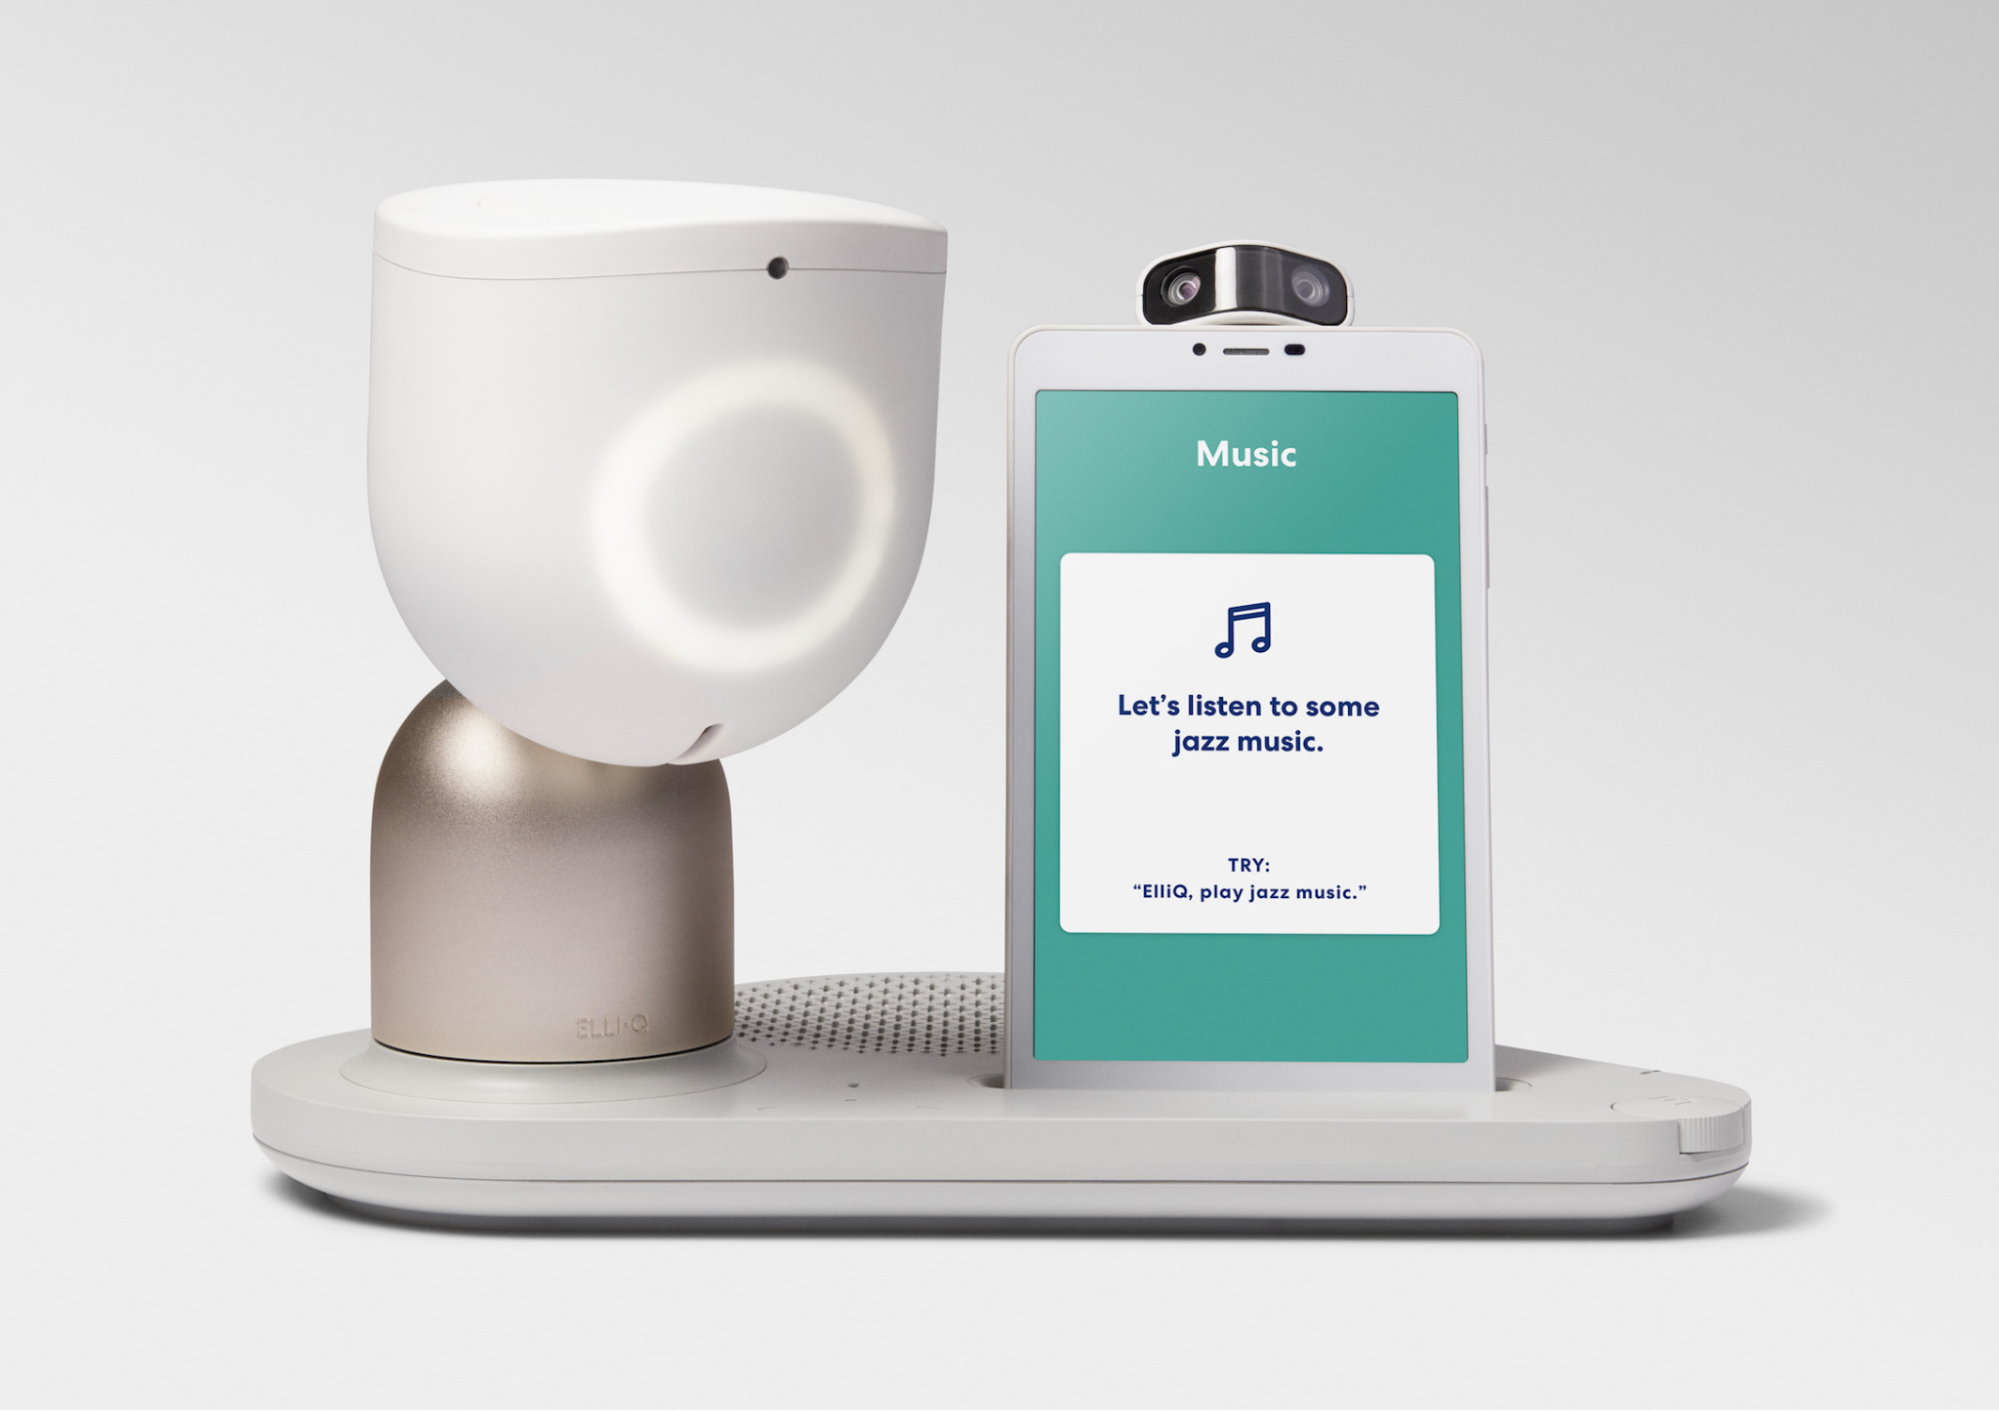
\includegraphics[width=0.6\textwidth]{elliq.png}
    \caption{ElliQ, Source: Adapted from \cite{ieee2023elliq}}
    \label{fig:elliq}
\end{figure}

\newpage
    \item{\bf{LOVOT}}
    \vspace{0.25cm}


LOVOT, developed by Groove X in Japan, is a social robot designed to provide companionship, particularly for older adults experiencing loneliness. Unlike stationary robots, LOVOT features a mobile, pet-like design equipped with AI-driven learning capabilities, allowing it to recognize users, respond to touch, and engage in affectionate interactions. The robot's design incorporates emotional expressiveness, including eye contact, physical warmth, and responsive movement, making it an appealing alternative to traditional social companionship.

A study by Tan et al. \cite{tan2024lovot} examined the impact of LOVOT on single older adults’ social well-being. Participants in the study interacted with LOVOT independently in their homes over a week and later shared their experiences in interviews. The study identified four key themes from these interactions: caring for the social robot, finding companionship, forming meaningful connections, and comparing the robot with traditional pets. Users reported that LOVOT provided emotional comfort and reduced feelings of loneliness, reinforcing the idea that social robots can serve as viable companions for older adults who live alone. Additionally, the participants expressed a preference for LOVOT over pets due to its lower maintenance requirements and its ability to provide companionship without the need for feeding or grooming.

LOVOT's adaptive AI enables it to tailor its behavior to individual users, reinforcing a sense of personal connection. This ability to form unique interactions based on user behavior sets LOVOT apart from other social robots. The study further emphasized the importance of designing robots that foster meaningful social engagement rather than serving as mere technological novelties. These findings suggest that social robots like LOVOT could play a crucial role in mitigating loneliness among aging populations and improving overall well-being.
\end{enumerate}


\begin{figure}[ht]
    \centering
    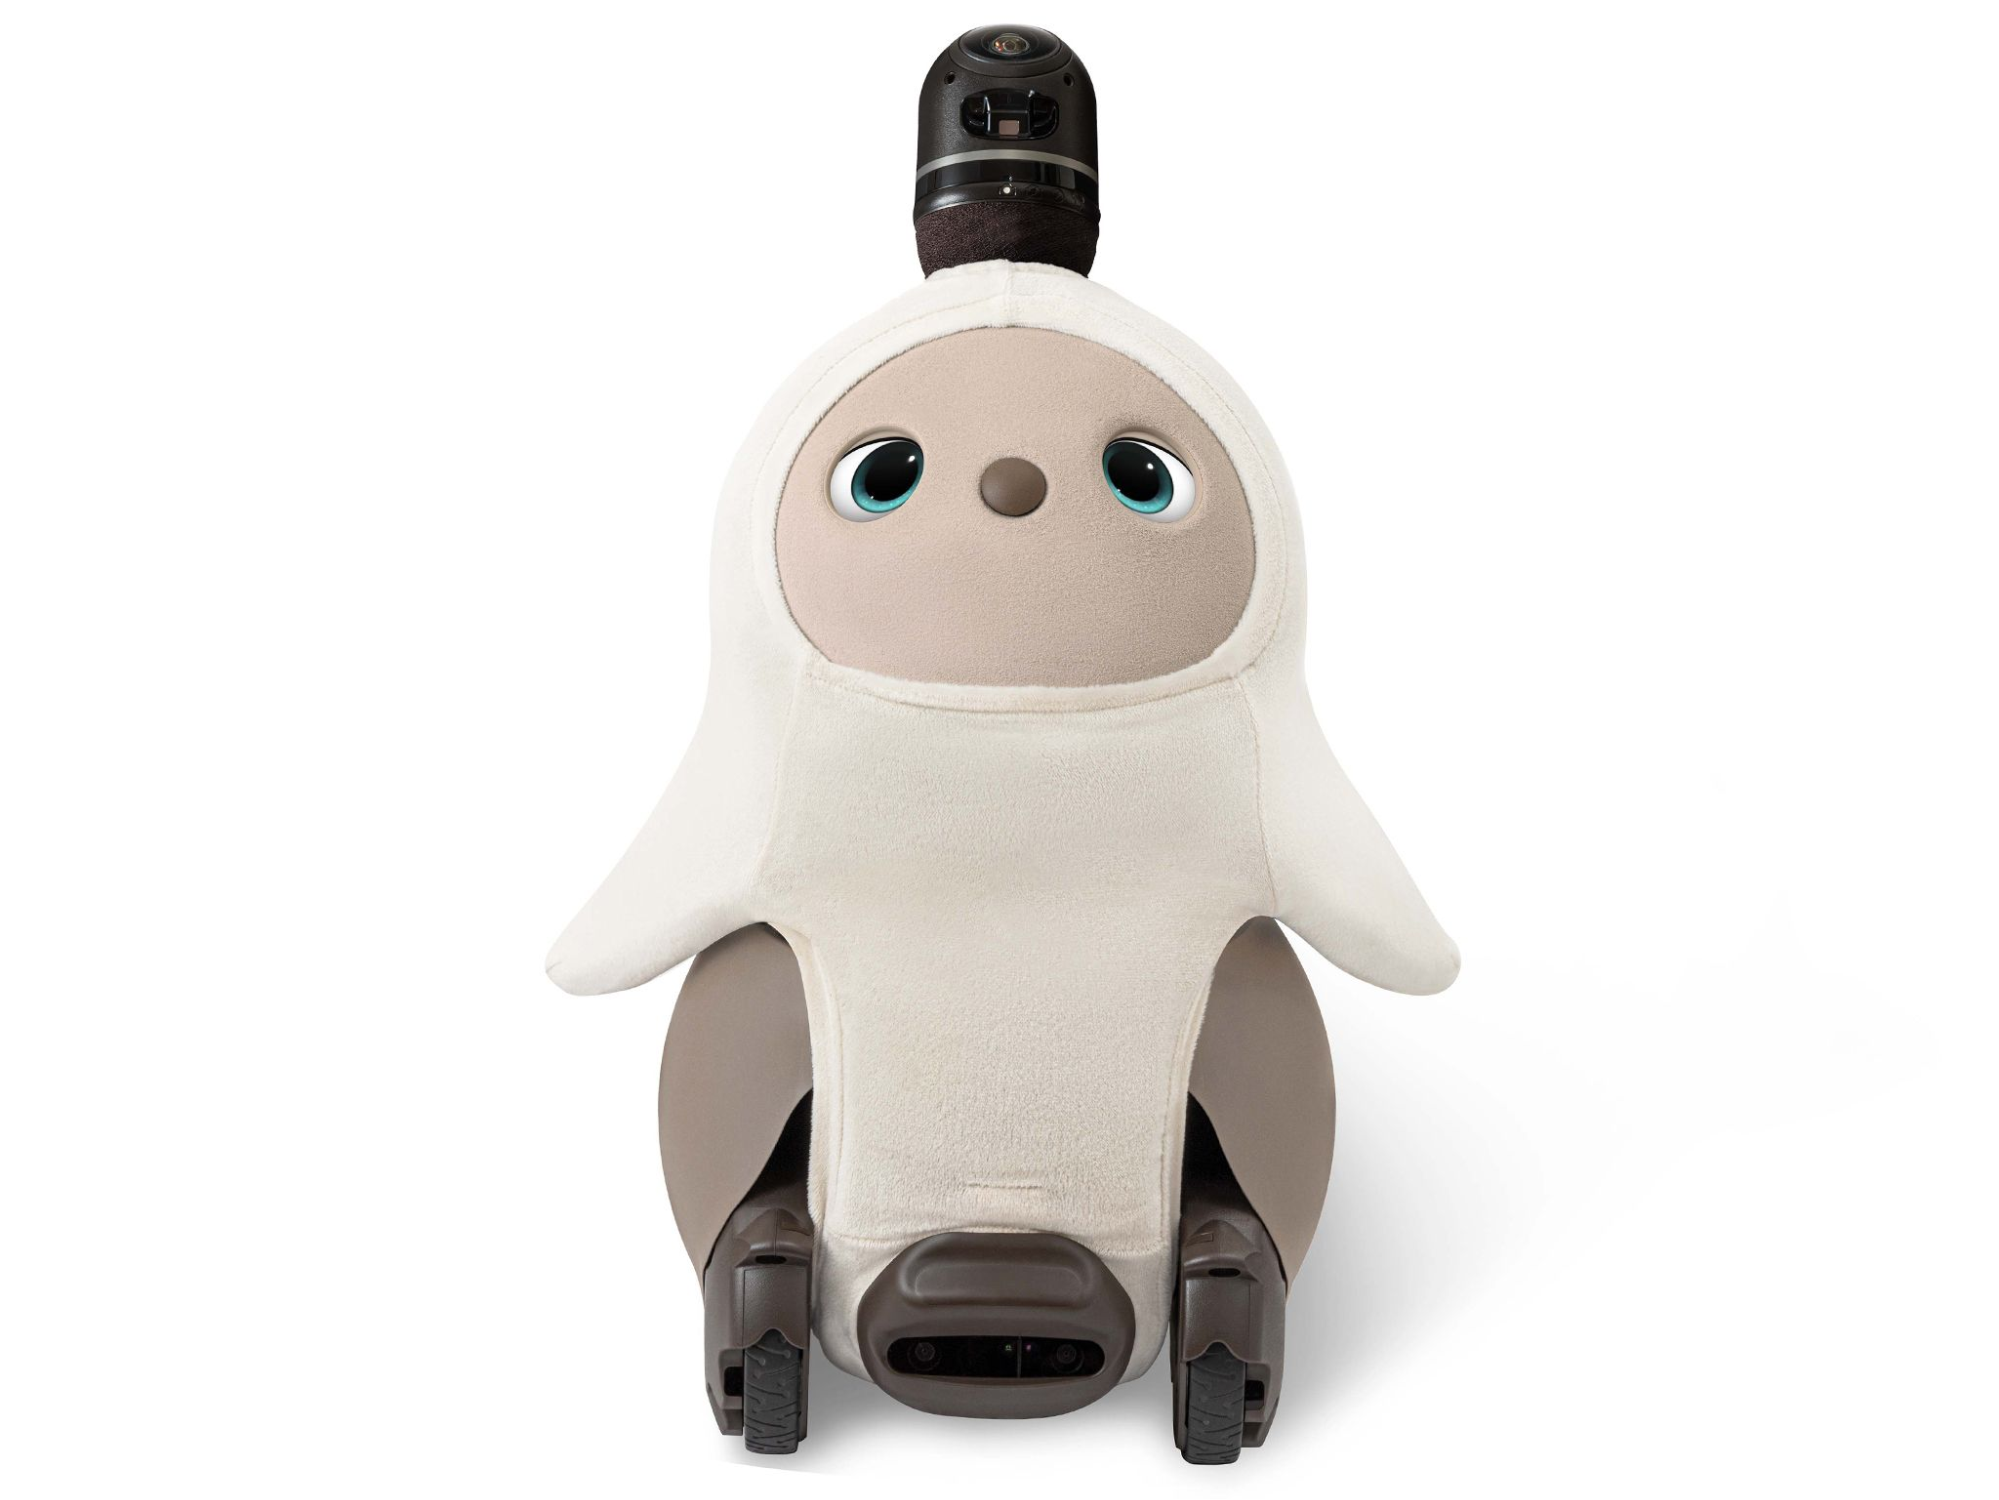
\includegraphics[width=0.6\textwidth]{lovot.png}
    \caption{LOVOT, Source: Adapted from \cite{lovot2024}}
    \label{fig:lovot}
\end{figure}

\subsection{State of the Art}

Bayesian Networks (BNs) are a proven tool for decision-making under uncertainty, as demonstrated by Rothmund et al. \cite{rothmund2021bayesian}, where Dynamic Bayesian Networks (DBNs) were applied to enhance the autonomy of industrial drones. The drones utilized DBNs to infer internal faults, assess environmental conditions, and make proactive decisions to avoid failures while executing independent tasks. By integrating information over time and dynamically updating beliefs, the drones optimized task execution while minimizing risks and the consequences of failures. Our project draws upon similar principles to develop a mental wellness robot designed to promote positivity and reduce stress. Although our robot operates with predefined action bubbles, which are structured interactions tailored to various user emotions, Bayesian Networks can play a vital role in determining which action bubble to deploy based on the user’s current emotional state.

Similar to the drone’s ability to assess environmental conditions, our robot can use a Bayesian Network to infer a user’s emotional state from multiple observable inputs such as facial expressions, vocal tone, and speech patterns. For instance, if vocal cues suggest frustration while facial expressions indicate neutrality, the Bayesian model can combine these observations to probabilistically identify the user’s dominant emotional state. Following the decision-making approach in the drone study, the Bayesian Network can evaluate which predefined action bubble, such as a greeting, playful movement, or verbal feedback, would most effectively promote wellness in the user. By assessing probabilistic relationships between input signals and predefined user emotions, the system ensures that interactions feel relevant and positive.

Emotional indicators are often incomplete or conflicting, such as vocal tone indicating stress while facial expressions suggest calmness. The Bayesian framework excels in such scenarios by integrating prior knowledge and real-time evidence to make confident decisions, ensuring that the robot’s interactions remain meaningful and appropriate. Rothmund et al. \cite{rothmund2021bayesian} emphasized the importance of minimizing risks in decision-making. Similarly, our robot uses Bayesian methods to weigh the likelihood of success for various action bubbles. For example, if the evidence suggests high uncertainty in emotional detection, the robot can select neutral or universally positive interactions to avoid a mismatch between the user’s needs and the robot’s response. The inclusion of Bayesian Networks ensures that the mental wellness robot adapts dynamically to user states, optimizing its responses to enhance emotional support and well-being.